\documentclass[12pt]{article}
\usepackage[margin=1in]{geometry} 
\usepackage{amsmath,amsthm,amssymb,amsfonts,enumerate,listings,graphicx,epstopdf}
\graphicspath{~/Documents/school/fall16/stat586/hw1}
 
\newcommand{\N}{\mathbb{N}}
\newcommand{\Z}{\mathbb{Z}}
 
\newenvironment{problem}[2][Problem]{\begin{trivlist}
\item[\hskip \labelsep {\bfseries #1}\hskip \labelsep {\bfseries #2.}]
  \vspace{1 cm}
}{\end{trivlist}}

\begin{document}
\title{Homework Set 1}
\author{Taylor Bodin}
\maketitle
 
\begin{problem}{2.1}
\item%{{{ 
    $N_{outcomes} = 5n+1$%}}}
\end{problem}

\begin{problem}{2.3}
  \item%{{{
  \begin{enumerate}[a.]
    \item The sample space forms a rectangle with vertices (0,0), (1,0), (1,2), and (0,2)
    \item The constraint forms an triangle with area .5. By geometric probability, $P(x \geq y) = \frac{1}{4}$
    \item Since there is no area contained under the line $x=y$, $P(x=y) = 0$
  \end{enumerate}%}}}
\end{problem}

\begin{problem}{2.5}
\item%{{{
  \begin{enumerate}[a.]
    \item 50
    \item $\frac{1}{5}$
    \item $\frac{7}{10}$
    \item $\frac{1}{10}$
  \end{enumerate}%}}}
\end{problem}

\newpage

\begin{problem}{2.7}
\item Assume $M = k+1$ %{{{
  \begin{align*}
    \textrm{let } p(x) &\equiv P\left( \bigcup_{i=1}^{x} A_i \right) = \sum_{i=1}^{x} A_i \\
    p(1) &\Rightarrow P(A_1) = P(A_1) & & \textrm{which is true by definition} \\
    p(2) &\Rightarrow P(A_1 \cup A_2) = P(A_1) + P(A_2) & & \textrm{which is true by axiom 2} \\
    \cdots \\
    p(M) &\Rightarrow p(k+1) = P\left( \bigcup_{i=1}^{k} A_i\ \cup A_{k+1} \right) = \sum_{i=1}^{M} A_i & & \textrm{then by axiom 2} \\
    p(M) &\Rightarrow P\left( \bigcup_{i=1}^{k} A_i\ \right) + P(A_{k+1}) = \sum_{i=1}^{M} A_i & & \textrm{which is true by definition}
  \end{align*}%}}}
\end{problem}

\begin{problem}{2.9}
  \begin{align*}%{{{
    P((A \cup B) \cup C) &= P(A \cup B) + P(C) - P((A \cup B) \cap C) \\
    &= P(A) + P(B) + P(C) - P(A \cap B) - P((A \cap C) \cup (B \cap C)) \\ 
    &= P(A) + P(B) + P(C) - P(A \cap B) - \left((P(A \cap C) + P(B \cap C) - P(A \cap B \cap C)\right) \\
    &= P(A) + P(B) + P(C) - P(A \cap B) - P(A \cap C) - P(B \cap C) + P(A \cap B \cap C) \\
  \end{align*}%}}}
\end{problem}

\begin{problem}{2.11}
  \begin{align*} %{{{
    \textrm{let }  P\left( \bigcup_{i=1}^M A_i \right) &= P\left( \bigcup_{i=1}^k A_i \cup A_{k+1} \right) & & \textrm{then by theorem 2.1} \\
    &= P\left( \bigcup_{i=1}^k A_i \right) + P(A_{k+1}) - P\left( \bigcup_{i=1}^k A_i \cap A_{k+1} \right) \\
    &= \sum_{i=1}^M P(A_i) - P\left( \bigcup_{i=1}^k A_i \cap A_{k+1} \right) \\
    \sum_{i=1}^M P(A_i) &\geq \sum_{i=1}^M P(A_i) - P\left( \bigcup_{i=1}^k A_i \cap A_{k+1} \right) & & \textrm{true by inspection} \\
  \end{align*}%}}}
\end{problem}

\newpage

\begin{problem}{2.13}
\item%{{{
  \begin{enumerate}[a.]
    \item
      \begin{itemize}
        \item Axiom 1: All probabilities are non-negative
        \item Axiom 2: $\frac{25}{64} + \frac{15}{54} + \frac{15}{64} + \frac{9}{64} = 1$
        \item Axiom 3: Since all the events are mutually exclusive with respect to one another, $P(\cup_1^4 A_i) = \sum_1^4 P(A_i)$
      \end{itemize}
    \item $\frac{5}{8}$
    \item $\frac{5}{8}$
  \end{enumerate}%}}}
\end{problem}

\begin{problem}{2.15}
\item%{{{
  \begin{enumerate}[a.]
    \item Axiom 1: Since the number of events can never be negative the first axiom holds
    \item Axiom 2: The sum of the individual events is equal to the toal number of trials, therefore axiom 2 holds
    \item Axiom 3: \\
      If A and B are mutually exclusive\dots \\
      \begin{align*}
        P(A) &= \frac{N_a}{N_{total}} \\
        P(B) &= \frac{N_b}{N_{total}} \\
        P(\bar{A} \cap \bar{B}) &= \frac{N_{neither}}{N_{total}} \\
        P(A \cap B) &= \frac{0}{N_{total}}
      \end{align*}
      Thus \\
      \begin{align*}
        P((\bar{A} \cap \bar{B}) \cup A \cup B)) &= \frac{N_{neither} + N_a + N_b}{N_{total}} = 1 \\
        P(A \cup B) &= \frac{1 - N_{neither} + N_a + N_b}{N_{total}}
      \end{align*}
      Therefore \\
      \begin{equation*}
        \frac{1-N_{neither}}{N_{total}} = \frac{N_a}{N_{total}} + \frac{N_b}{N_{total}} = P(A) + P(B)
      \end{equation*}
  \end{enumerate}%}}}
\end{problem}

\newpage

\begin{problem}{2.17}
\item Instead, assume that the spinner comes to rest from $[0,2\pi)$ to form an angle between the spinner and an arbitrary reference point. We%{{{
    could then assign probabilities to each of the numbers based on how wide their sector is. %}}}
\end{problem}

\begin{problem}{2.19}
\item $P(x = n) = \frac{1}{2}^{n-1}(\frac{1}{2}) = \frac{1}{2}^n$%{{{
\end{problem}%}}}

\begin{problem}{2.21}
\item%{{{
  \begin{enumerate}[a.]
    \item Axiom 1: If $P(A \cap B)$ and $P(B)$ are valid and $P(B) \neq 0$, $P(A|B) \geq 0$
    \item Axiom 2: \\
      \begin{align*}
        P(A|B) + P(A^c|B) &= 1 \\
        \frac{P(A \cup B)}{P(B)} + \frac{P(A^c|B)}{P(B)} &= 1 \\
        \frac{P(A\cup A^c)\cap P(B)}{P(B)} &= 1 \\
        \frac{P(S)\cap P(B)}{P(B)} &= 1 \\
        \frac{P(B)}{P(B)} &= 1 \\
        1 &= 1
      \end{align*}
    \item Axiom 3: The conditional probability of mutually exculisve events is 0 which is a valid probability
  \end{enumerate}%}}}
\end{problem}

\begin{problem}{2.23}
  \begin{align*}%{{{
    P(D_1 \cup D_2) &= 1 - P(\bar{D_1} \cup \bar{D_2}) \\
    &= 1 - \frac{5}{30}\frac{5}{29} \\
    &= \frac{9}{29}
  \end{align*}%}}}
\end{problem}

\newpage

\begin{problem}{2.25}
\item %{{{
  \begin{enumerate}[a.]
    \item $\frac{5}{6}\frac{5}{6} = \frac{25}{36}$
    \item By counting: $\frac{6}{36}$
    \item $P(3)\cap P(5) \cup P(5)\cap P(3) = \frac{1}{6}\frac{1}{6} + \frac{1}{6}\frac{1}{6} = \frac{2}{36}$
    \item $P(5)\cap(P(5)\cup P(4)) = \frac{1}{6}\frac{2}{6} = \frac{2}{36}$
    \item By counting $\frac{1}{36}$
    \item $P(6) \cup P(6) \cup P(6 \cap 6) = \frac{1}{6} + \frac{1}{6} + \frac{1}{36} = \frac{11}{36}$
  \end{enumerate}%}}}
\end{problem}

\begin{problem}{2.27}
\item Given that $P(A) > P(B)$\dots%{{{
  \begin{align*}
    P(A|B) &> P(B|A) \\
    \frac{P(A\cap B)}{P(B)} &> \frac{P(A\cap B)}{P(A)} & & \textrm{Which is true except when A and B are mutually exculsive}
  \end{align*}%}}}
\end{problem}

\begin{problem}{2.77}
\item%{{{
  \lstinputlisting{problem_2_77.m}%}}}
\end{problem}

\newpage

\begin{problem}{2.79}
\item%{{{
  \begin{figure}[htpb]
    \centering
    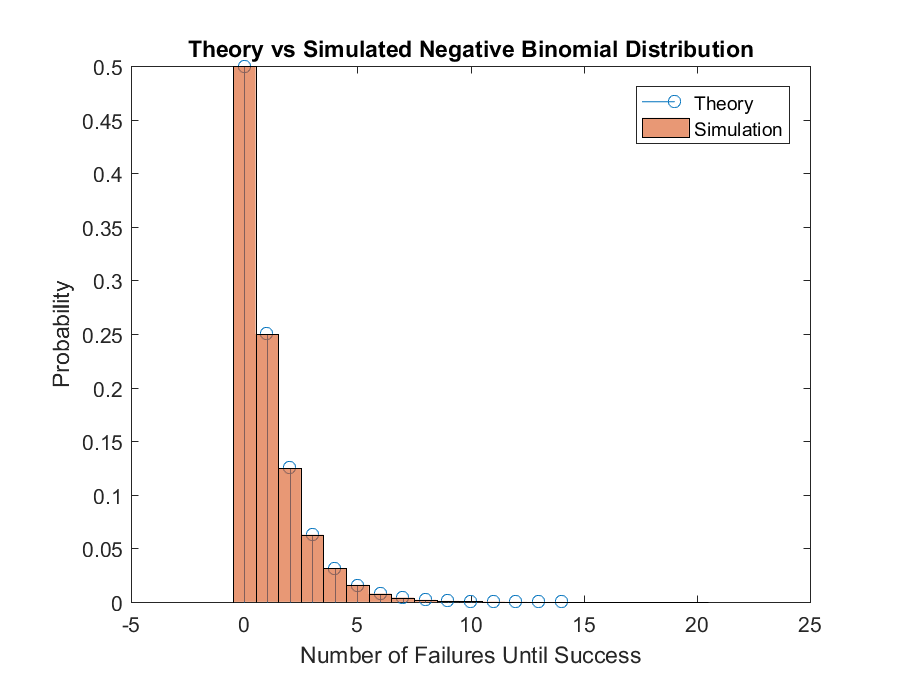
\includegraphics[scale=1]{fig_2_79.eps}
    \caption{Problem 2.79, Simulation of the Negative Binomial Distribution}
  \end{figure}%}}}
\end{problem}

\end{document}
